\section{Browser comparison and user-supplied execution images}
\label{sec:browser}

\subsection{Shared model and generation path}

The current WGSL branch serves a comparison page with two backends: CPU WebAssembly and WebAssembly with WGSL matrix products.  Both use the same checkpoint, Wasm tokenizer, Wasm sampler, FP32-to-FP64 sampling adapter, and generation loop.  The CPU choice loads \code{model-cpu.wasm}, the unchanged parent module copied into the bundle.  The WGSL choice loads the hybrid \code{model.wasm} and six shader files.  The comparison action runs CPU WebAssembly first and WGSL second with the same prompt and settings~\cite{browser-source,wg-packedguide}.

Each run creates a worker.  The hybrid path also creates a WebGPU device and shared transfer staging.  The worker performs model calls and keeps the weights and cache in the module's linear memory.  When a matrix import runs, it copies the input vector to staging and posts the requested matrix role and weight offsets.  The host dispatches a shader, reads its output, copies the bytes to staging, and signals the worker.  The worker resumes after the completion signal and copies those bytes into the allocated Wasm result.  This implements a synchronous import over the browser's asynchronous GPU API~\cite{browser-source}.

The GPU host prepares raw-word weight views on demand.  A linear view appends the bias vector to its matrix words.  A vocabulary view transposes the tied embedding slice into the shader's expected indexing.  Those operations rearrange bytes and words.  Model arithmetic executes in the Wasm module and shaders.  The host retains the views for later token calls and destroys the device when the run ends.  The model uses fifty views: four for each of twelve layers and two for the vocabulary slices~\cite{browser-source,wg-packedsource}.

The page compares generated token IDs and the stopping reason.  It retains both displayed completions and reports whether they agree.  At temperature zero the shared sampler selects greedily.  The visible seed remains part of the settings, while the greedy path determines the displayed run's selection rule.  Matching token IDs establishes that the two paths selected the same continuation on that run.  The visible comparison records token agreement.  Exact logit equality remains a separate test property~\cite{browser-source,wg-packedguide}.

\subsection{Completion shown in the first image}

Figure~\ref{fig:browser-completion} reproduces \code{gpt-1.png}, supplied by Jamie Stephens on 19 September 2026 after a run of the WGSL branch web demonstration.  The prompt is
\begin{quote}
[Bad fiction contest] It was a dark and stormy night as
\end{quote}
The requested completion length is 32 tokens, the temperature is zero, and the seed is 42.  The selected WebGPU option is ``Available GPU.''  The displayed adapter identifies vendor \code{apple} and architecture \code{metal-3}.  These labels identify the API-reported adapter information visible in the screenshot.  The screenshot provenance record accompanies the image file~\cite{screenshots}.

Both result panes show the same continuation:
\begin{quote}
we were walking down the street. I was standing in the middle of the street, and I saw a man with a gun. I thought, 'What the
\end{quote}
The page reports that both runs finished after 32 generated tokens because the requested count was reached.  The continuation therefore ends at the generation limit shown by the interface.  It demonstrates execution through model calls, token selection, and text decoding for this prompt.  The formal inference result addresses the model's cache and logits at the encoded-token interface described earlier.

\begin{figure}[p]
\centering
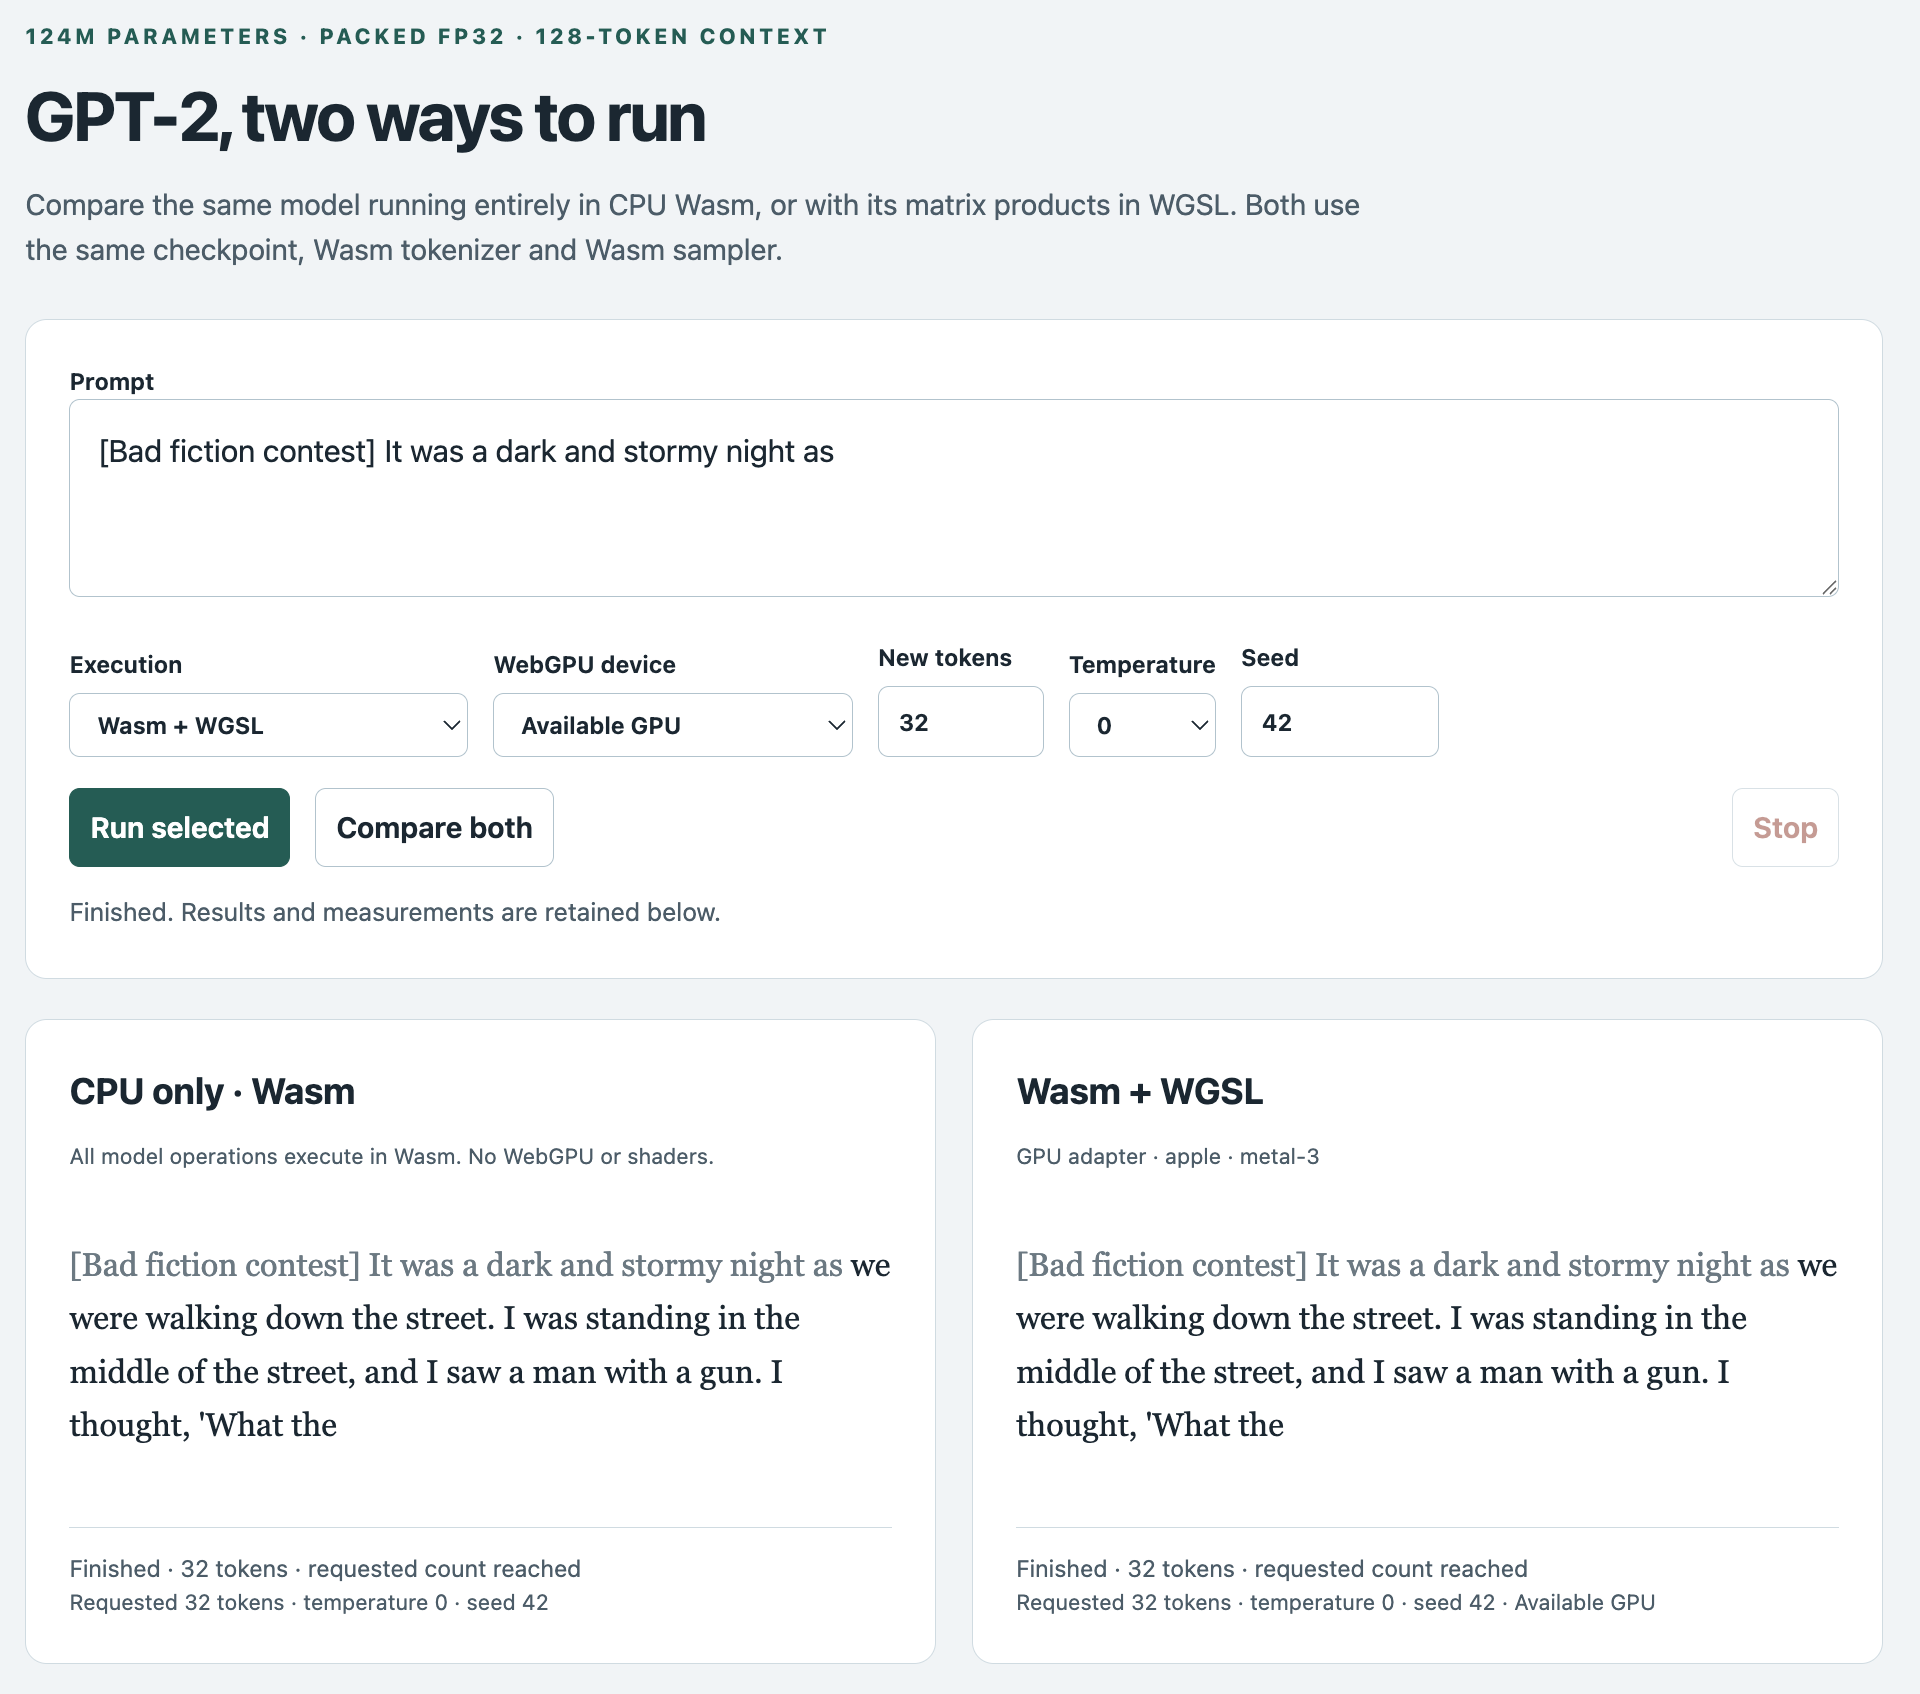
\includegraphics[width=\linewidth,height=0.85\textheight,keepaspectratio]{figures/gpt-1.png}
\caption{User-supplied browser completion comparison.  CPU WebAssembly and the hybrid Wasm/WGSL path show the same 32-token greedy continuation.  Settings, adapter labels, completion text, and stopping status remain visible.  The original image is included without content edits.}
\label{fig:browser-completion}
\end{figure}

\subsection{Timing definitions and the second image}

Figure~\ref{fig:browser-measurements} reproduces \code{gpt-2.png} from the same reported demonstration.  It records fourteen prompt tokens, thirty-two generated tokens, and thirty-one subsequent decode model steps for each backend.  The first generated token uses the logits produced by the final prompt call.  Each later generated token requires another model call.  Consequently, the decode-throughput numerator is 31 in this run~\cite{screenshots,browser-source}.

Prefill processes prompt tokens one at a time.  The reported prefill rate divides the number of completed prompt tokens by time spent in those model calls.  CPU WebAssembly takes 5.533 seconds at a displayed 2.53 tokens/s.  The hybrid takes 0.545 seconds at 25.71 tokens/s.  The corresponding elapsed-time ratio is approximately 10.15 using the displayed rounded durations.  The model-call timing includes host transfer and waiting time for WGSL.  Lazy creation and upload of weight views occur during prefill~\cite{screenshots,browser-source}.

Decode takes 11.820 seconds on CPU WebAssembly and 0.752 seconds on the hybrid path.  The displayed rates are 2.62 and 41.23 model steps/s.  The page reports a 15.72-fold ratio from its measurements.  Ratios recomputed from the rounded durations or rounded rates can differ in the last displayed digits.  These values describe the observed continuation and this implementation's timing definitions~\cite{screenshots}.

Setup takes 0.269 and 0.253 seconds.  The host measures setup from the start of a run through device and pipeline preparation, module and asset loading, tokenization, and worker readiness as applicable to the backend.  The first-token metric then begins after setup and ends at the worker's first token emission.  The displayed first-token times are 5.535 and 0.546 seconds.  Total elapsed time includes setup and is 17.647 seconds for CPU WebAssembly and 1.567 seconds for the hybrid path, a ratio of approximately 11.26 from the displayed numbers~\cite{screenshots,browser-source}.

Sampling and text-decoding counters have their own timed regions.  The image reports sampling times of 0.008 and 0.006 seconds and text-decoding times of 0.016 and 0.011 seconds.  The generation-elapsed measurement also contains loop, messaging, and other intervening work.  The backend comparison therefore supports a statement about complete generation and model-call throughput in addition to the selected kernel implementation~\cite{screenshots,browser-source}.

\begin{figure}[p]
\centering
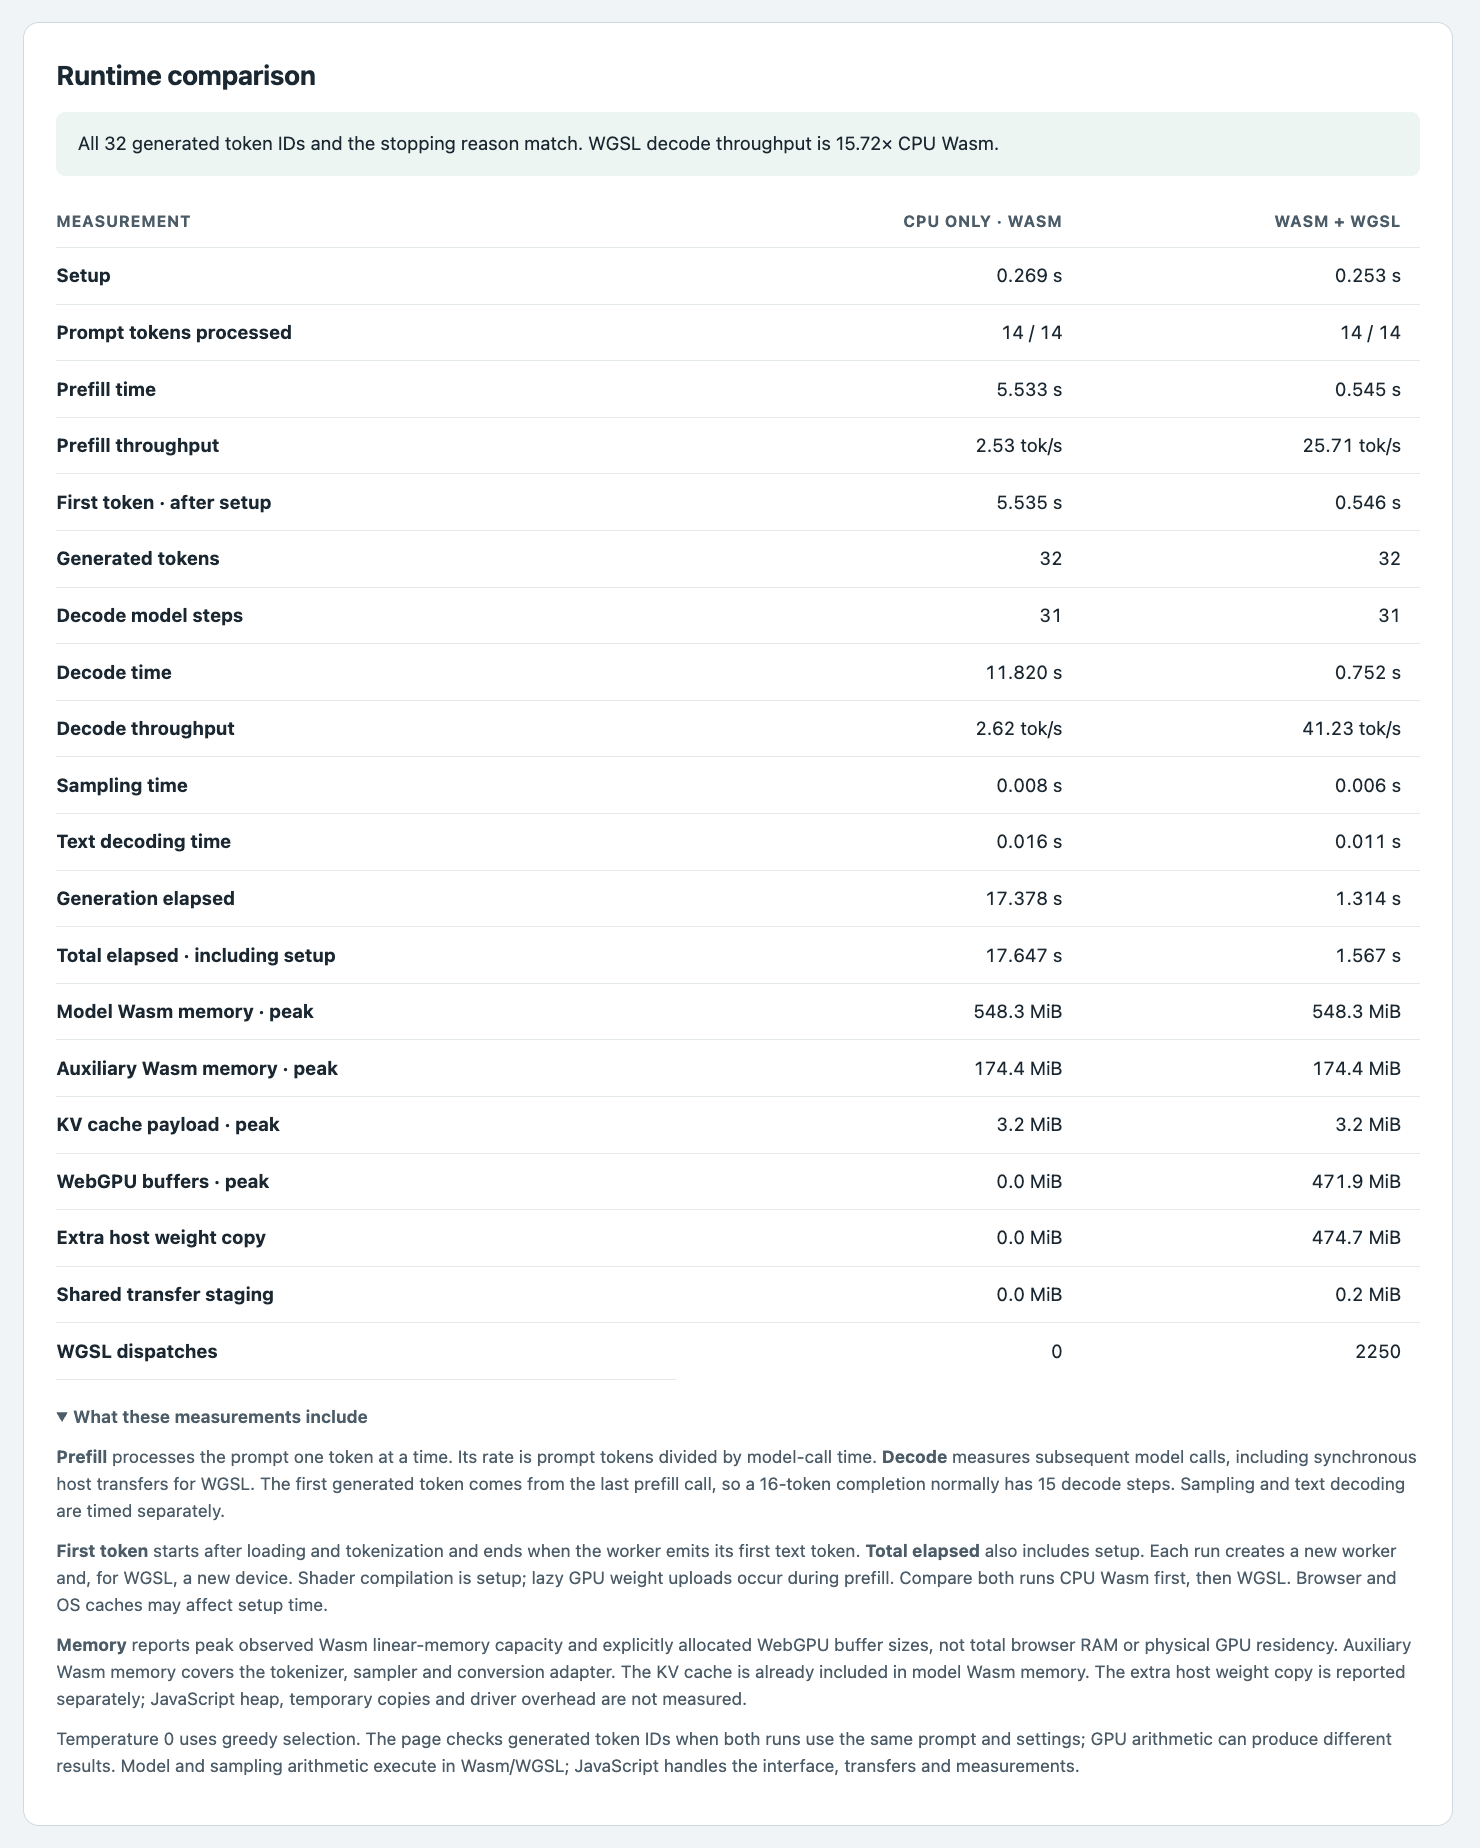
\includegraphics[width=\linewidth,height=0.87\textheight,keepaspectratio]{figures/gpt-2.png}
\caption{User-supplied runtime comparison for the completion in Figure~\ref{fig:browser-completion}.  The page reports matching token IDs and stopping reason, a 15.72-fold decode-throughput ratio, and separate timing, memory-capacity, and dispatch counters.  The explanatory text at the bottom defines the measurements.  The original image is included without content edits.}
\label{fig:browser-measurements}
\end{figure}

\subsection{Memory accounting and dispatch count}

The image reports peak model Wasm linear-memory capacity of 548.3 MiB for both paths and auxiliary Wasm capacity of 174.4 MiB.  The auxiliary total covers the tokenizer, sampler, and conversion adapter.  The 3.2 MiB peak key/value payload occupies part of the model memory.  Adding it again to model capacity would double-count those bytes.  These counters describe represented buffer capacities at observed points in the run~\cite{screenshots,browser-source}.

The hybrid path also reports 471.9 MiB of allocated WebGPU buffers, a 474.7 MiB host weight copy, and 0.2 MiB of shared staging.  The host weight-copy size follows from the 497,759,232-byte checkpoint.  The device buffers contain selected matrix views and transfer buffers.  The two paths can therefore have equal model linear-memory capacities while retaining different additional memory.  Physical GPU residency, JavaScript heap usage, temporary upload copies, browser internals, and driver allocations require other measurements~\cite{screenshots,browser-source}.

The dispatch count has a direct explanation in the source.  Four matrix shaders run per transformer layer and two shaders cover the vocabulary projection, giving
\[
12\times4+2=50
\]
dispatches per model call.  This run makes fourteen prefill calls and thirty-one decode calls, giving
\[
(14+31)\times50=2250.
\]
That value equals the image's reported dispatch count.  The cache payload after forty-five calls has $45\times73{,}728=3{,}317{,}760$ bytes, which rounds to the displayed 3.2 MiB.  These consistency checks relate the UI counters to the implemented call structure~\cite{screenshots,browser-source}.

\subsection{Experimental interpretation and provenance}

The screenshots provide a user-recorded browser completion and timing observation.  The retained evidence consists of the two original PNG files, their hashes, the visible settings and results, the user's environment description, and the inspected measurement source at the WGSL checkpoint.  The user identifies the browser as Chrome and the machine as a Mac mini with a 10-core CPU, a 10-core GPU, 32 GB of memory, 1 TB of storage, and Gigabit Ethernet.  The images contain the Apple/Metal adapter labels.  The Chrome version, chip model, and identity of the executed bundle remain unrecorded.  The report attributes the run and machine description to the user and the timing definitions to the inspected source~\cite{screenshots,browser-source}.

The fixed run order gives the second backend a different cache history.  Each run creates a fresh worker and, for WGSL, a fresh device, but browser and operating-system asset caches can persist between runs.  Pipeline preparation and weight upload also occur in different timed regions.  The displayed decode comparison includes the hybrid's synchronous transfer and wait costs, which makes it useful as a measurement of this complete model-call path.  Repeated trials with recorded versions and varied order would be needed to characterize variability or a wider hardware population~\cite{browser-source}.

The browser run extends the earlier report's execution evidence.  At the pinned branch checkpoint, the development journal still records browser execution as pending after automation failures.  It separately records a Node execution of the real CPU worker, matching sixteen selected tokens and 804,112 logit words against a native trace, plus cancellation and cleanup checks.  Those worker tests and the supplied browser images have different provenance.  This report retains both and identifies the screenshots as the new browser observation~\cite{wg-journal,browser-tests,screenshots}.

The browser CPU engine also differs from the Wasmtime configuration used by the native theorem application.  The strict formal arithmetic includes a selected arithmetic NaN word.  Applying that exact raw-word guarantee to browser WebAssembly requires evidence for the browser's arithmetic behavior on the relevant domain.  The hybrid adds the shader arithmetic and transfer premises described in Section~\ref{sec:hybrid}.  Matching text and token IDs in the displayed run supports that run's observed behavior.  Establishing those premises for every permitted weight array requires a stronger runtime correspondence result.
